\documentclass[oneside,a4paper,14pt]{extarticle}
\usepackage[a4paper,letterpaper,top=20mm,bottom=20mm,left=20mm,right=10mm]{geometry}
\usepackage[russian]{babel}
\usepackage{indentfirst}
\usepackage{graphicx}
\usepackage{caption}
\usepackage{titlesec}
\usepackage{minted, fancyvrb}

\titleformat{\section} {\normalsize\bfseries} {\thesection} {1em} {}
\titleformat{\subsection} {\normalsize\bfseries} {\thesubsection} {1em} {}
\titleformat{\subsubsection} {\normalsize\bfseries} {\thesubsection} {1em} {}
\renewcommand\baselinestretch{1.45}\normalsize
\setlength{\parindent}{1.25cm}

\begin{document}

\newpage
\thispagestyle{empty}
\begin{center}
	МИНИСТЕРСТВО НАУКИ И ВЫСШЕГО ОБРАЗОВАНИЯ РОССИЙСКОЙ ФЕДЕРАЦИИ ФЕДЕРАЛЬНОЕ ГОСУДАРСТВЕННОЕ БЮДЖЕТНОЕ ОБРАЗОВАТЕЛЬНОЕ УЧРЕЖДЕНИЕ ВЫСШЕГО ОБРАЗОВАНИЯ\\
	«ВЯТСКИЙ ГОСУДАРСТВЕННЫЙ УНИВЕРСИТЕТ»\\
	Институт математики и информационных систем\\
	Факультет автоматики и вычислительной техники\\
	Кафедра электронных вычислительных машин
\end{center}
\vspace{10mm}

\hfill
\begin{tabular}{l}
	\footnotesize Дата сдачи на проверку:                                          \\
	\footnotesize <<\rule[-1mm]{5mm}{0.10mm}\/>>\rule[-1mm]{20mm}{0.10mm}\ 2025 г. \\
	\footnotesize Проверено:                                                       \\
	\footnotesize <<\rule[-1mm]{5mm}{0.10mm}\/>>\rule[-1mm]{20mm}{0.10mm}\ 2025 г. \\
\end{tabular}
\vfill

\begin{center}
	РЕАЛИЗАЦИЯ ЭЛЕМЕНТАРНЫХ СТРУКУР ДАННЫХ НА ОСНОВЕ ДИНАМИЧЕСКОЙ ПАМЯТИ\\
	Отчёт по лабораторной работе №6\\
	по дисциплине\\
	<<Программирование>>\\
\end{center}
\vspace{25mm}
\noindent
\begin{tabular}{ll}
	Разработал студент гр. ИВТб-1301-05-00 & \rule[-1mm]{30mm}{0.10mm}\,/Черкасов А. А./   \\
	                                       & \hspace{8mm}\footnotesize(подпись)            \\
	Заведующая кафедры ЭВМ                 & \rule[-1mm]{30mm}{0.10mm}\,/Долженкова М. Л./ \\
	                                       & \hspace{8mm}\footnotesize(подпись)            \\
\end{tabular}

\noindent
\begin{tabular}{lp{58mm}r}
	Работа защищена &  & <<\rule[-1mm]{5mm}{0.10mm}\/>>\rule[-1mm]{30mm}{0.10mm}\ 2025 г.
\end{tabular}
\vfill

\begin{center}
	Киров\\
	2025
\end{center}

\newpage\thispagestyle{plain}

\section*{Цель}

Цель работы: Изучение структуры и принципов организации программных модулей, закрепление навыков работы с динамической памятью. Получение базовых навыков организации работы в режиме командной строки.

\section*{Задание}
\begin{itemize}
	\item[$-$] Написать программу для работы со структурой данных "Кольцевой двусвязный список".
	\item[$-$] Структура данных должна быть реализована на основе динамической памяти.
	\item[$-$] Структура данных (поля и методы) должна быть описана в отдельном модуле.
	\item[$-$] Работа со структурой должна осуществляться в режиме командной строки (с реализацией автодополнения и истории команд).
	\item[$-$] Предусмотреть наглядную визуализацию содержимого структуры.
\end{itemize}

\section*{Решение}

Схемы алгоритмов решения задач представлена на рисунках 1 и 2. Исходный код решений представлен в Приложениях А1 и А2.

\clearpage
\begin{figure}[H]
	\centering
	% 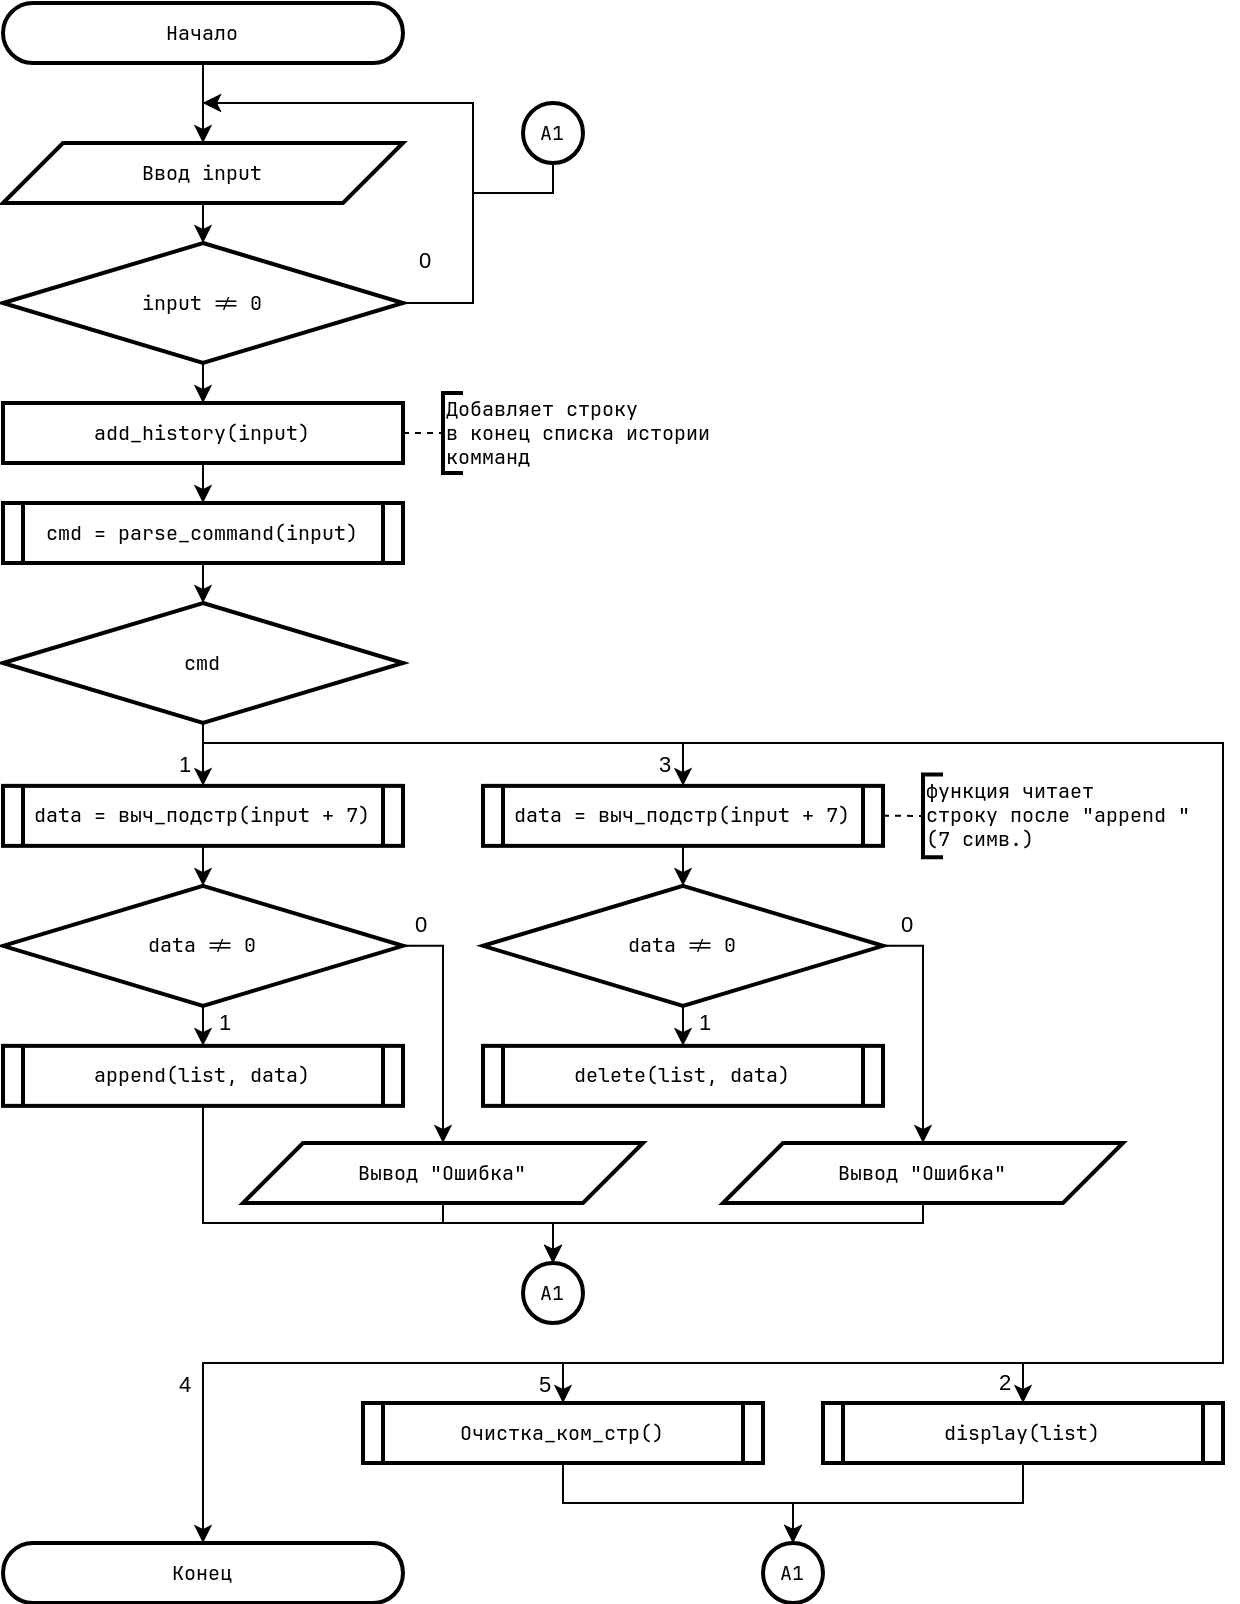
\includegraphics[height=0.9\textheight]{pics/flowchart1.png}
	\caption*{Рисунок 1 - Схема алгоритма Задания 1.}
\end{figure}

\begin{figure}[H]
	\centering
	% 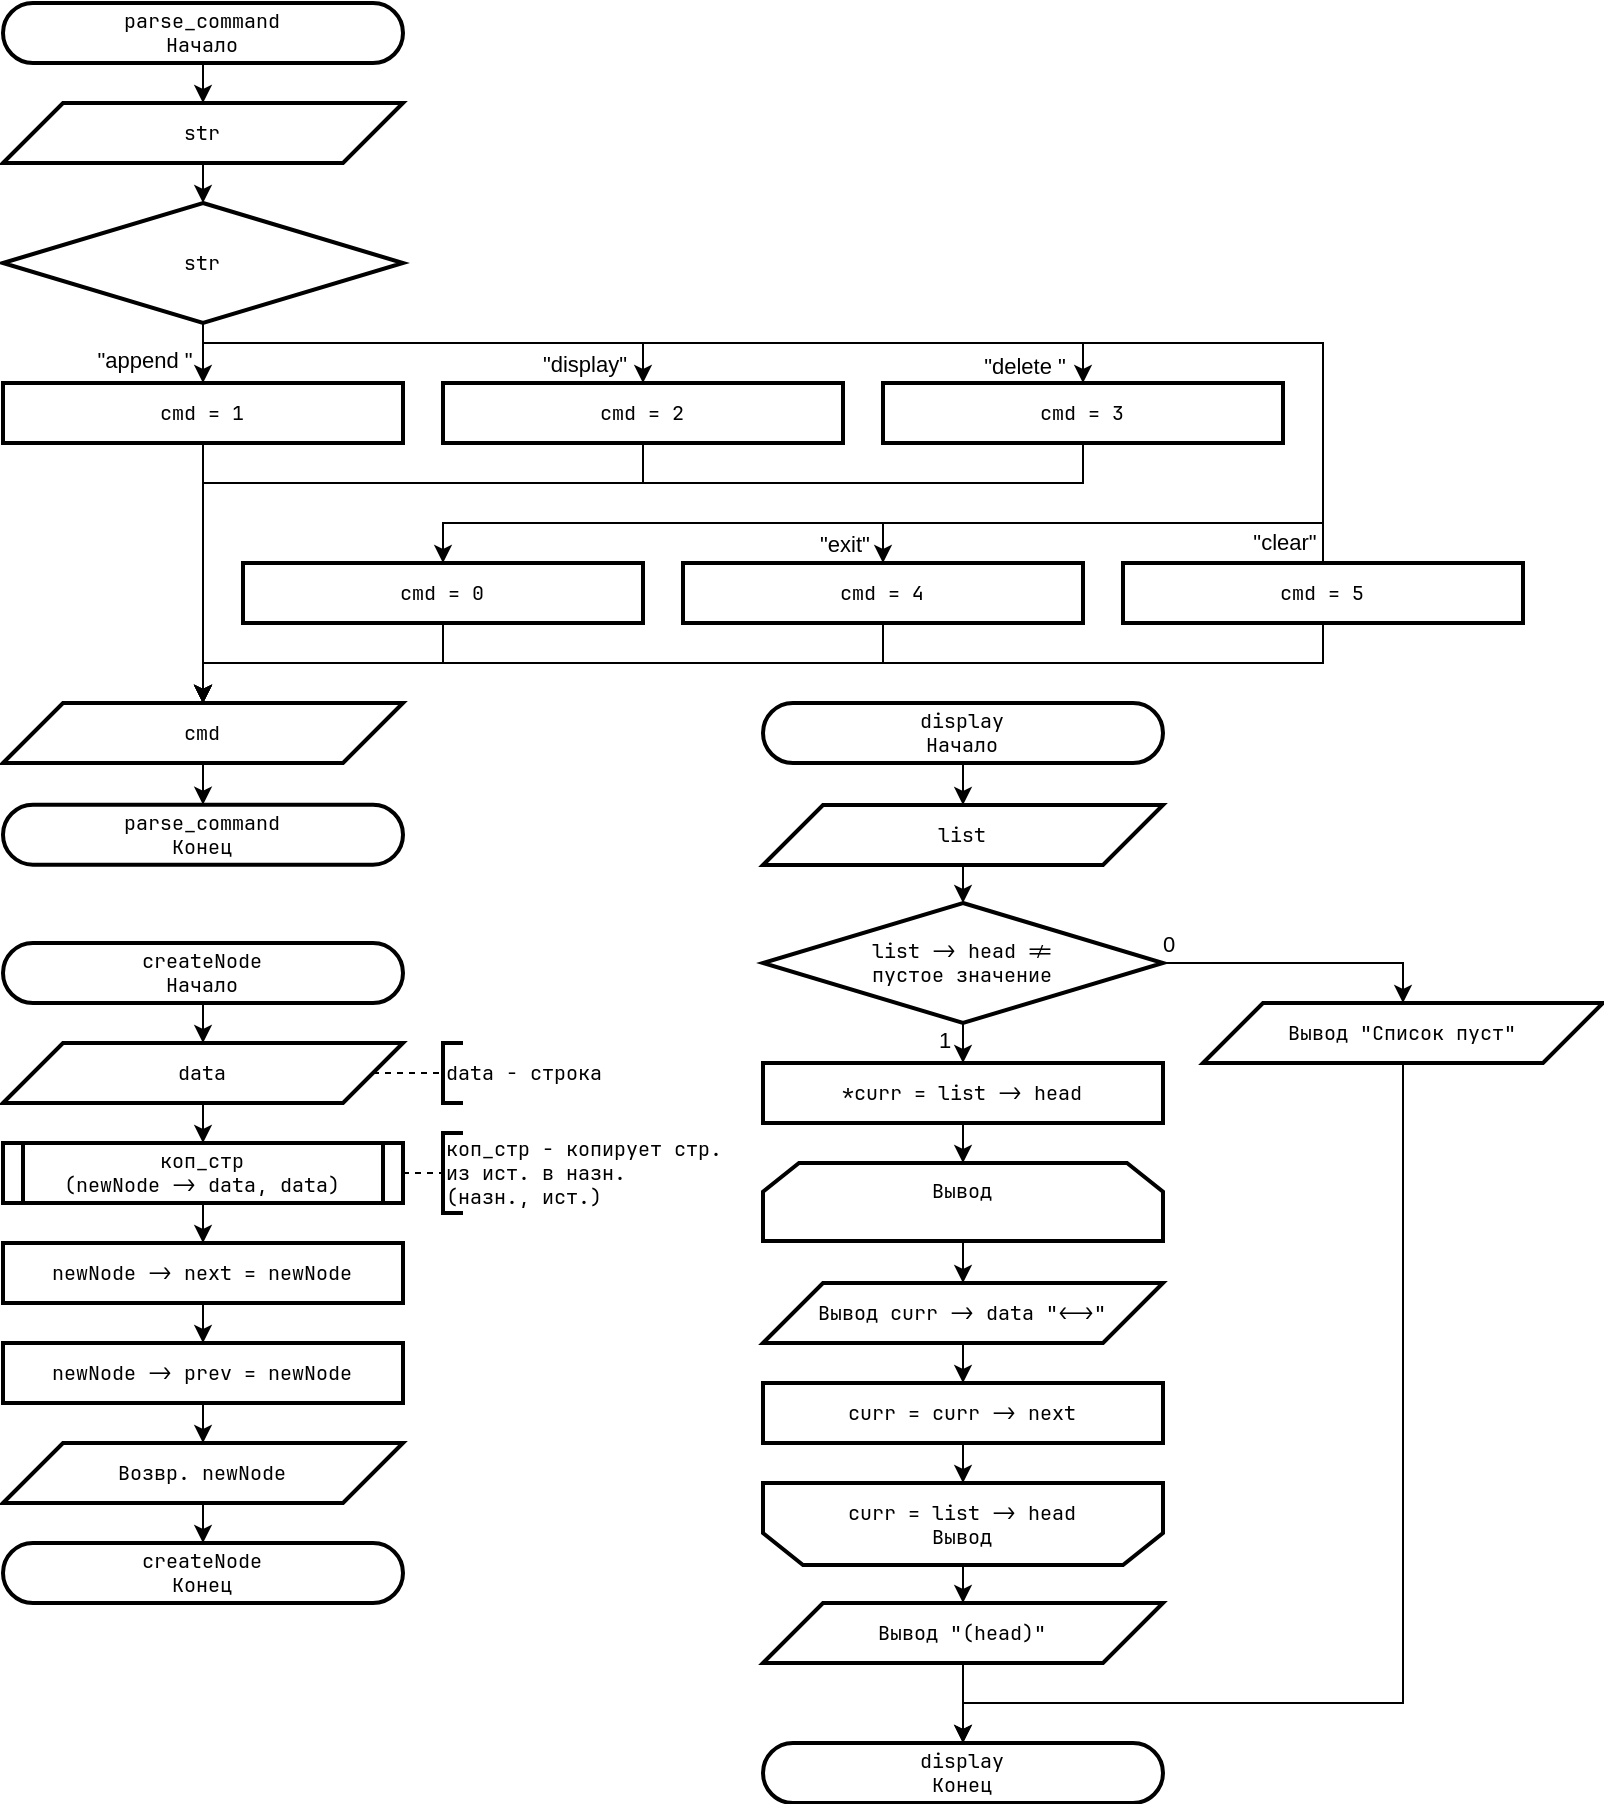
\includegraphics[height=0.9\textheight]{pics/flowchart2.png}
	\caption*{Рисунок 2 - Схема алгоритма Задания 2.}
\end{figure}

\section*{Вывод}

\setminted{style = rainbow_dash, fontsize = \small} % https://pygments.org/styles/

В результате работы были реализована консольная программа для работы со структурой "Кольцевой двусвязный список" с использованием программных модулей.

\newpage

\section*{Приложение А1. Исходный код}
\inputminted{cpp}{code/cdll.h}

\section*{Приложение А2. Исходный код}
\inputminted{cpp}{code/cdll.c}

\section*{Приложение А3. Исходный код}
\inputminted{cpp}{code/cli.c}

\end{document}
